\section{Zielsetzung}
\label{sec:zielsetzung}
In dotierten Ionenkristallen treten Dipole auf.
Diese werden in diesem Versuch, mit dem Ziel deren Anregungsenergie $W$ und
charakteristische Relaxationszeit $τ_0$ zu ermitteln, untersucht.

\section{Theoretische Grundlagen}
\label{sec:theorie}
\subsection{Dipole in dotierten Ionenkristallen}
Die hier verwendete Kaliumbromid-Probe ist ein Ionenkristall,
dieser besteht aus einem regelmäßigen Gitter aus
Kalium-Kationen und Brom-Anionen (Abb. \ref{fig:probeBild}).
\FloatBarrier
\begin{figure}
    \centering
    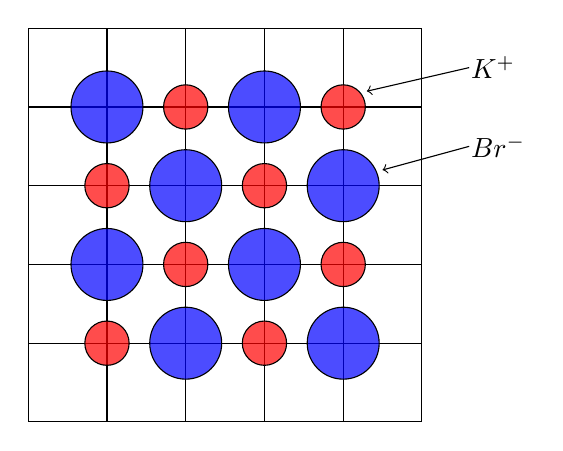
\begin{tikzpicture}
        %grid
        \draw[step=1.0,black,thin] (0,0) grid (5,5);
        %ions
        \filldraw[fill opacity=0.7, fill=red] (1,1) circle (8pt);
        \filldraw[fill opacity=0.7, fill=blue] (2,1) circle (13pt);
        \filldraw[fill opacity=0.7, fill=red] (3,1) circle (8pt);
        \filldraw[fill opacity=0.7, fill=blue] (4,1) circle (13pt);
        \filldraw[fill opacity=0.7, fill=blue] (1,2) circle (13pt);
        \filldraw[fill opacity=0.7, fill=red] (2,2) circle (8pt);
        \filldraw[fill opacity=0.7, fill=blue] (3,2) circle (13pt);
        \filldraw[fill opacity=0.7, fill=red] (4,2) circle (8pt);
        \filldraw[fill opacity=0.7, fill=red] (1,3) circle (8pt);
        \filldraw[fill opacity=0.7, fill=blue] (2,3) circle (13pt);
        \filldraw[fill opacity=0.7, fill=red] (3,3) circle (8pt);
        \filldraw[fill opacity=0.7, fill=blue] (4,3) circle (13pt);
        \filldraw[fill opacity=0.7, fill=blue] (1,4) circle (13pt);
        \filldraw[fill opacity=0.7, fill=red] (2,4) circle (8pt);
        \filldraw[fill opacity=0.7, fill=blue] (3,4) circle (13pt);
        \filldraw[fill opacity=0.7, fill=red] (4,4) circle (8pt);
        %nodes
        \draw (5.5, 4.5) node[right] {$K^{+}$};
        \draw[->] (5.6, 4.5) -- (4.3, 4.2); 
        \draw (5.5, 3.5) node[right] {$Br^{-}$};
        \draw[->] (5.6, 3.5) -- (4.5, 3.2);
    \end{tikzpicture}
    \caption{Form eines KBr Ionenkristalls.}
    \label{fig:probeBild}
\end{figure}

\FloatBarrier
Kalium ist ein Alkalimetall (1te~Hauptgruppe) und Brom ist ein Halogen
(7te~Hauptgruppe). Der gesamte Kristall ist somit elektrisch neutral.

Der Kristall ist mit Strontium ($\ce{Sr^{2+}}$) dotiert.
Dies führt dazu, dass eine negative Ladung (Elektron) fehlt.
Im Kristall bildet sich so ein Dipol aus.
Diese sind bei Raumtemperatur statistisch so verteilt, dass das
Gesamtdipolmoment des Kristalls null ist.

\subsection{Depolarisationseffekte}
Als Vorgriff auf die Durchführung [\ref{sec:durchfuehrung}] sei hier erwähnt,
dass die Dipole in der Probe erst mit einem von außen angelegtem E-Feld
ausgerichtet und dann in diesem Zustand eingefroren werden.
Anschließend wird die Probe langsam wieder erwärmt
und der Strom in der Probe gemessen.
Dieser Strom stammt aus der Reorientierung der Dipole, die bei ansteigender
Temperatur wieder in die Ausgangslage relaxieren.

Der Abstand zwischen dem zweifach geladenen Ion und der Kationen-Leerstelle gibt die Richtung des Dipols an, sodass aufgrund
der Gitterplätze nur diskrete Dipolrichtungen im Kristall vorliegen können.
Unter $\SI{500}{\celsius}$ ist eine Richtungsänderung der Dipole nur durch eine Leerstellendiffusion möglich, welche unter einer
materialspezifischen Aktivierungsenergie $W$ auftritt.
Der Anteil der Dipole, welche durch thermische Bewegung diese Energie aufbringen können, ist durch die Boltzmann-Statistik gegeben
und somit proportional zu $\exp{\left(-W/k_\text{B}T\right)}$.
Daraus folgt für die Relaxationszeit eines Dipols der Zusammenhang

\begin{equation}
    \tau(T) = \tau_0 \exp\!\left(\frac{W}{k_\text{B}T}\right)
    \label{eqn:relax}
\end{equation}

mit der charakteristischen Relaxationszeit $\tau_0 = \tau(\infty)$.
\\~\\
Theoretisch kann der Depolarisationsstrom mittels zwei Ansätzen beschrieben werden:

\subsection{Polarisationsansatz}

Der Depolarisationsstrom ist im allgemeinen
\begin{equation}
    i(T) = -\frac{\mathrm{d}P(t)}{\mathrm{d}t}\,.
    \label{eqn:polstrom2}
\end{equation}

Die Polarisationsrate hängt von der übrigen Polarisation zur Zeit $t$
und von der Relaxationsrate $\tau(T)$ ab.
\begin{equation}
    \frac{\dif{P(t)}}{\dif{t}} = -\frac{P(t)}{\tau(T)}
    \label{eqn:polrate}
\end{equation}

Einsetzen von Gleichung \eqref{eqn:polrate} in Gleichung \eqref{eqn:polstrom2} ergibt

\begin{equation}
    i(T) = \frac{P(t)}{\tau(T)}\,.
    \label{eqn:i_t_polstart}
\end{equation}

Nach Integration von Gleichung \eqref{eqn:polrate} erhält man einen Zusammenhang für $P(t)$.

\begin{equation}
    P(t) = P_{0} \exp\!\left(-\frac{t}{\tau(T)}\right)\,,
\end{equation}

welcher sich mit Gleichung \eqref{eqn:i_t_polstart} zu

\begin{align}
    i(T) &= \frac{P_0}{\tau} \exp\!\left(-\frac{t}{\tau(T)}\right) \\
    \intertext{bestimmt. Die Zeit $t$ kann nun als Integral geschrieben werden,
    vom Zeitpunkt des abschalten des elektrischen Feldes zum Beginn des Depolarisationsstroms}
    i(T) &= \frac{P_{0}}{\tau}
    \exp\!\left(-\int_0^t \frac{\dif{t}}{\tau(T)}\right)\,. \\
\end{align}

Nimmt man nun eine konstante Heizrate b mit

\begin{equation}
    b := \frac{\dif{T}}{\dif{t}} = \text{const}
    \label{eqn:heiz}
\end{equation}

an, nimmt der Depolarisationsstrom die Form

\begin{equation}
    i(T) = \frac{P_0}{\tau} \exp\!\left(-\int_{T_0}^T
      \exp\!\left(- \frac{W}{k_B T}\right) \dif{T}\right)
\end{equation}

an.

\subsection{Stromdichtenansatz}

Aus dem Debye-Modell für hohe Temperaturen erhalten wir die mittlere Polarisation\cite{polarisation} $\bar{\symup{P}}(T)$ als

\begin{equation}
    \bar{\symup{P}}(T) = \frac{N}{N_V}\frac{p^2 E}{3k_B T}\,,
\end{equation}

wobei $p$ das Dipolmoment beschreibt, $E$ das elektrische Feld und $T$ die Temperatur.
Die Dichte der Dipole wird mit $N_V$ erfasst.
Die Änderung der Anzahl $N$ an Dipolen, die in der Zeit $t$ relaxieren, ist ein
thermisch aktivierter Prozess,
wird also durch Temperaturerhöhung gefördert und lässt sich schreiben als

\begin{equation}
    \frac{\dif{N}}{\dif{t}} = -\frac{N}{\tau(T)}\,.
    \label{eqn:dNdt}
\end{equation}

Dabei ist

\begin{equation*}
    N = N_\mathrm{P} \exp\!\left( -\frac{1}{b} \int_{T_0}^T
      \frac{\dif{T'}}{\tau(T')} \right)
    \label{eqn:anzahlDipole}
\end{equation*}

mit $N_\mathrm{P}$ als Zahl der zu Beginn des Aufheizens vorhandenen orientierten Dipole pro Volumeneinheit
und somit ergibt sich für den Depolarisationsstrom $i(T)$, welcher sich auch als Rate an Dipolrelaxationen verstehen lässt

\begin{equation}
    i(T) = \bar{\symup{P}}(T) \frac{\dif{N}}{\dif{t}}\,.
    \label{eqn:polstrom}
\end{equation}

Aus Gleichung \eqref{eqn:dNdt} und Gleichung \eqref{eqn:polstrom} erhält man so eine geschlossene Formel für den Depolarisationsstrom.

\begin{equation}
    i(T) = -\bar{P}(T) \frac{\symup{N}}{\tau(T)}\,.
\end{equation}

Einsetzen von allen bekannten Termen ergibt
\begin{equation}
    i(T) = \frac{ p^2 E }{ 3 k_\mathrm{B} T_\mathrm{P} } \frac{ N_\mathrm{P} }{ \tau_0 } \exp{ \left( - \frac{ 1 }{ b \tau_0 }
    \int_{T_0}^T \exp{ \left( - \frac{ W }{ k_\mathrm{B} T' } \right) \mathrm{d}T' } \right) } \exp{
    \left( -\frac{ W }{ k_\mathrm{B} T } \right) }
    \label{eqn:i_t}
\end{equation}

wobei $b$ die Heizrate ist.

\subsection{Berechnung der Aktivierungsenergie $W$}
\label{sub:W_A}
\subsubsection{Bestimmung mithilfe des Maximums}

Im ersten Verfahren ist das Integral in Gleichung \eqref{eqn:i_t} etwa

\begin{equation*}
    \int_{T_0}^T \exp{ \left( - \frac{ W }{ k_\mathrm{B} T } \right )} \approx 0 \,,
\end{equation*}

woraus sich der Strom näherungsweise als

\begin{equation}
    \label{eqn:approx}
    i(T) \approx \frac{ p^2 E }{ 3 k_\mathrm{B} T_\mathrm{P} } \frac{ N_\mathrm{P} }{ \tau_0 } \exp{ \left( - \frac{ W }{ k_\mathrm{B} T}
    \right ) }
\end{equation}

schreiben lässt.
Durch anwenden des Logarithmus ergibt sich eine Geradengleichung für $i(T)$ gegen $\frac{1}{T}$ zu

\begin{equation}
    \symup{ln}\left(i(T)\right) = \underbrace{\left(\frac{p^{2} E N_{p}}{3 k_{B} T \tau_{0}}\right)}_{\text{const.}} \underbrace{-\frac{W}{k_{B}}}_{\text{Steigung}} \frac{1}{T}\,.
\end{equation}

Die Aktivierungsenergie ergibt sich also zu

\begin{equation}
    W = m \cdot k_{B}
\end{equation}

wobei m die Steigung der Geraden ist.

\subsubsection{Verwendung des gesamten Kurvenverlaufs}

Die zweite Methode verwendet die gesamte Stromkurve. Für die Gesamtpolarisation gilt

\begin{equation}
    \frac{\mathrm{d}P}{\mathrm{d}t} = \frac{ P(t) }{ \tau(T(t))}\,.
    \label{eqn:dPdt1}
\end{equation}

Der durch die Änderung der Polarisation hervorgerufene Strom hängt vom Probenquerschnitt $F$ gemäß

\begin{equation}
    \frac{\mathrm{d}P}{\mathrm{d}t} = \frac{i(t)}{F} \,.
    \label{eqn:dPdt2}
\end{equation}

ab.
Wird die Gleichung \eqref{eqn:dPdt1} nach $\tau(T)$ umgestellt und mit
$\frac{\mathrm{d}T}{\mathrm{d}T}$ erweitert, folgt

\begin{align}
    \tau(T) &= P(T) \cdot \frac{\mathrm{d}T}{\frac{\mathrm{d}P}{\mathrm{d}t} \mathrm{d}T }\,.
    \intertext{Mit Gleichung \eqref{eqn:heiz} wird $\tau$ zu}
    \tau(T) &= \frac{P(t) \mathrm{d}T}{b \mathrm{d}P}\,.
    \intertext{Erweitern mit $\frac{\mathrm{d}t}{\mathrm{d}t}$ liefert nun}
   \tau(T) &= \frac{P(t)}{b} \frac{\mathrm{d}T}{\mathrm{d}P}\frac{\mathrm{d}t}{\mathrm{d}t}
           = \frac{P(t)}{b} \frac{\frac{\mathrm{d}T}{\mathrm{d}t}}{\frac{\mathrm{d}P}{\mathrm{d}t}}
   \intertext{Mit der Definition aus Gleichung \eqref{eqn:dPdt2} und umschreiben der Polarisation als $P = \int \mathrm{d}P$ erhält man}
   \tau(T) &= \frac{\int \frac{\mathrm{d}P}{\mathrm{d}t}\mathrm{d}T}{i(T) b}
\end{align}

Nun erh\"alt man mit Gleichung \eqref{eqn:dPdt2} die Darstellung für $\tau(T)$

\begin{equation*}
    \tau(T) = \frac{ \int_{T}^\infty i(T') \mathrm{d}T' }{ i(T) b}
\end{equation*}

und durch ersetzen von $\tau(T)$

\begin{equation}
    \label{eqn:integrate}
     W = k_\mathrm{B} T \ln{ \left( \frac{ \int_{T}^\infty i(T') \mathrm{d}T' }{ i(T) b\tau_0 } \right) } \,,
\end{equation}

woraus sich nun $W$ berechnen lässt.
In der Praxis wird die obere Integrationsgrenze von $\infty$ in $T^*$ geändert, wobei $j(T^*) \approx 0$ gilt.

\subsection{Berechung der charakeristischen Relaxationszeit}

Um die charakterische Relaxationszeit zu erhalten differenziert man Gleichung \eqref{eqn:i_t} nach der Zeit.

\begin{equation}
    \frac{\mathrm{d}i(T)}{\mathrm{d}T} \propto \frac{1}{\tau_{0}} \left( -\frac{1}{b\tau_{0}} \int_{T_{0}}^{T}
    \exp\frac{W}{k_{B}T} \mathrm{d}T' - \frac{W}{k_{B}T} \right) \left( \frac{W}{k_{B}T^{2}} - \frac{ 1 }{ b \tau_{0} }
    \left( \exp -\frac{W}{k_{B} T} \right) \right)\,.
    \label{di_dt}
\end{equation}

Es folgt für $\tau$ in Abhängigkeit der Maximaltemperatur

\begin{equation}
    τ_0 = τ\l(T_{\text{max}}\r) \exp\!\!\left(-\frac{W}{k_b T_{\text{max}}}\right)
     = \frac{k_{B}T^{2}_{\text{max}}}{W b}
      \exp\!\!\left(-\frac{W}{k_b T_{\text{max}}}\right)\,.
    \label{eqn:theo-tau}
\end{equation}
